\documentclass[compress]{beamer}
\usepackage{setspace}
\usepackage{multicol}
\mode<presentation>
{
  %\usetheme{Warsaw}
  %\usecolortheme{spruce}
  % or ...
	%\useoutertheme{infolines}
  %\setbeamercovered{transparent}
  
  \usetheme{CambridgeUS}
    \setbeamercolor{item projected}{bg=darkred}
    \setbeamertemplate{enumerate items}[default]
    \setbeamertemplate{navigation symbols}{}
    \setbeamercovered{invisible}
    \setbeamercolor{block title}{fg=darkred}
    \setbeamercolor{local structure}{fg=darkred}
  
  % or whatever (possibly just delete it)
}

\usepackage{verbatim} 
\usepackage{listings}
\usepackage{tikz}
\usetikzlibrary{arrows}
\usetikzlibrary{shapes}
\tikzstyle{block}=[draw opacity=0.7,line width=1.4cm]

\newcommand{\bigpause}{\bigskip \pause}
\newcommand\azul[1]{{\color{blue}#1}}
\lstloadlanguages{C++}
\lstnewenvironment{code}
	{%\lstset{	numbers=none, frame=lines, basicstyle=\small\ttfamily, }%
	 \csname lst@SetFirstLabel\endcsname}
	{\csname lst@SaveFirstLabel\endcsname}
\lstset{% general command to set parameter(s)
	language=C++, basicstyle=\footnotesize\sffamily, keywordstyle=\slshape,
	emph=[1]{tipo,usa}, emphstyle={[1]\sffamily\bfseries},
	basewidth={0.47em,0.40em},
	columns=fixed, fontadjust, resetmargins, xrightmargin=5pt, xleftmargin=15pt,
	flexiblecolumns=false, tabsize=2, breaklines,	breakatwhitespace=false, extendedchars=true,
	numbers=left, numberstyle=\tiny, stepnumber=1, numbersep=9pt,
	frame=l, framesep=3pt,
}

\usepackage[spanish]{babel}
% or whatever

\usepackage[utf8]{inputenc}

\usepackage{graphicx}
\usepackage{caption}
\usepackage{multirow}
\usepackage{subcaption}

\usepackage{times}
\usepackage[T1]{fontenc}
% Or whatever. Note that the encoding and the font should match. If T1
% does not look nice, try deleting the line with the fontenc.


\title[Análisis y predicción de la búsqueda visual humana] % (optional, use only with long paper titles)
{Análisis y predicción de la búsqueda visual humana}

\author[Melanie Sclar] % (optional, use only with lots of authors)
{~Melanie Sclar}
% - Give the names in the same order as the appear in the paper.
% - Use the \inst{?} command only if the authors have different
%   affiliation.
\institute[UBA] % (optional, but mostly needed)
{
  %\inst{1}%
  Facultad de Ciencias Exactas y Naturales\\
  Universidad de Buenos Aires
}
%\date[PAP] % (optional, should be abbreviation of conference name)
%{Problemas, Algoritmos y Programación}

% Delete this, if you do not want the table of contents to pop up at
% the beginning of each subsection:
\AtBeginSubsection[]
{
  \begin{frame}<beamer>{Contenidos}
    \tableofcontents[currentsection,currentsubsection]
  \end{frame}
}

%\newcommand{\be}{\begin{equation*}}
\newcommand{\ee}{\end{equation*}}
\newcommand{\state}[1]{\left|\,#1\,\right\rangle}
\newcommand{\costate}[1]{\left\langle\,#1\,\right|}
\newcommand{\trace}{\text{Tr}}
\newcommand{\su}{\uparrow}
\newcommand{\sd}{\downarrow}
\newcommand{\im}{\text{Im}}
\newcommand{\re}{\text{Re}}

% If you wish to uncover everything in a step-wise fashion, uncomment
% the following command:

%\beamerdefaultoverlayspecification{<+->}


\begin{document}
\pgfdeclarelayer{background}
\pgfsetlayers{background,main}
\begin{frame}
  \titlepage
\end{frame}

\section{Introducción}
\begin{frame}{Agudeza visual}
\begin{itemize}
\item Podemos ver en detalle solo una pequeña porción del campo visual, aquella que cae en un área de la retina llamada \textit{fóvea}.
\item Debido a las limitaciones de agudeza en la retina, los movimientos oculares son necesarios para procesar detalles.
\end{itemize}
\end{frame}

\begin{frame}{Movimientos oculares}
\begin{itemize}
\item Existen dos categorías básicas de movimientos oculares: las sacadas y las persecuciones suaves.
\item Los ojos rotan rápidamente para fijar la vista en una nueva posición y centrar la fóvea. Este proceso ocurre varias veces por segundo sin involucrar la consciencia de las personas.
\end{itemize}
\end{frame}

\begin{frame}
\begin{center}
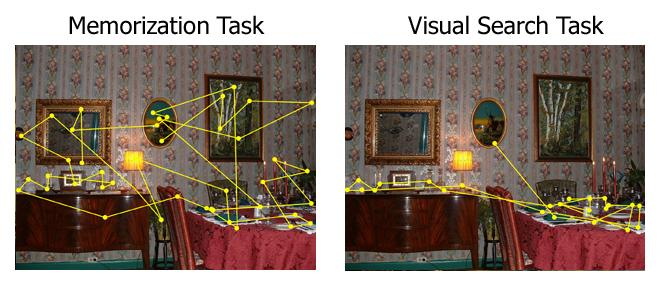
\includegraphics[width=0.8\textwidth]{images/castelhano-fixations.jpg}
\end{center}

Las ubicaciones de las fijaciones no son aleatorias y los patrones que describen dependen fuertemente de la tarea que realice. Aún si no damos ninguna tarea en particular, las personas miran en puntos que les resultan más informativos.
\end{frame}

\begin{frame}{Modelos de saliencia}

\begin{itemize}
\item Como no podemos procesar toda la información de una imagen a la vez, restringimos los procesos complejos a un área reducida que es considerada interesante. 
\item Después, analizamos distintas regiones una atrás de la otra. 
\item ¿Cómo decidimos qué región seleccionar para captar nuestra atención primero?
\item Este es el problema de decidir qué regiones son más salientes, y desde la computación se crean \textbf{mapas de saliencia} que predicen estas regiones.
\end{itemize}

\end{frame}

\begin{frame}{Modelos de saliencia (2)}
\begin{center}
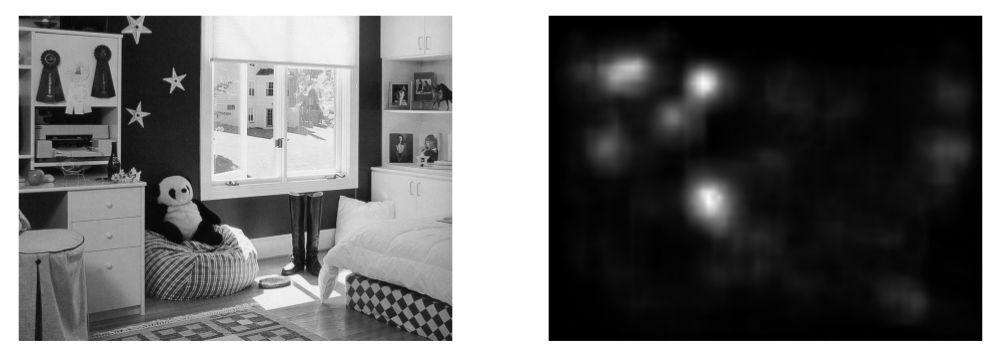
\includegraphics[width=0.9\textwidth]{images/ejemplo-mlnet.png}
\end{center}

{\small Los mapas de saliencia aún no logran reproducir a la perfección los lugares de la imagen que más llaman la atención humana, pero año a año hay avances en este área.\\}

\bigskip

{\small En \texttt{http://saliency.mit.edu/} hay una recopilación de los mejores modelos a la fecha. De ahí, tomamos tres: Judd, SAM y MLNet.}

\end{frame}

\begin{frame}
\begin{itemize}
\item Los modelos de saliencia toman en cuenta diferentes factores que afectan la atención visual, como ser los colores, el contraste, la orientación, la presencia de texto o humanos, entre otros.
\item Estos factores se clasifican en dos categorías: \textit{bottom-up} (dependiendo únicamente de las características de la imagen) y \textit{top-down} (dependiendo de la tarea que se realice).
\end{itemize}
\end{frame}

\begin{frame}{Búsqueda visual}
% definir búsqueda visual?
En la búsqueda visual se combinan factores \textit{top-down} y \textit{bottom-up}, de tal forma que a veces regiones muy salientes se ignoran porque son poco relevantes para la tarea.

\bigskip
La saliencia suele funcionar mejor en escenas artificiales que en naturales, porque en estos últimos afectan también factores contextuales y semánticos.

\bigskip

Esto no significa que la saliencia deje de ser relevante, pero se suele combinar ésta con mapas más específicos como detectores de target o un mapa de apariencia esperada del target.

\end{frame}

% pasar para más adelante
\begin{frame}{Modelos de movimientos oculares en imágenes}
\end{frame}

\begin{frame}{Métricas de comparación de \textit{scanpaths}}
No hay consenso sobre qué métrica utilizar para comparar scanpaths, ya que hay muchos factores a tener en cuenta. Así, algunos de los más famosos son:
\begin{itemize}
\item Cantidad de fijaciones hasta encontrar el target
\item Edit distance de strings, con variaciones según las operaciones que se permitan: inserción, eliminación o sustitución de un caracter.
% edit distance lo explico con un ejemplo en el pizarrón 
\item Ángulos entre fijaciones
\item Distancia de Mannan
\end{itemize}
\end{frame}

\begin{frame}{Creación de un corpus de interiores}
\begin{itemize}
\item Recolectamos 134 imágenes de interiores de $768 \times 1024$ píxeles.
\item Las imágenes son en blanco y negro y no tienen personas ni texto.
\item Recortamos varios targets por imagen de diferentes y seleccionamos al azar uno por imagen, siempre y cuando fuera menor a $72 \times 72$.
\item Luego uniformizamos los targets para que todos tengan $72 \times 72$ píxeles.
\end{itemize}
\end{frame}

\begin{frame}{Diseño del experimento de búsqueda visual}

\begin{itemize}
\item Utilizamos un Eye Tracker para grabar los movimientos oculares del ojo derecho. Los participantes solo pueden mover la vista y no la cabeza durante el experimento.
\item Realizamos 134 ensayos, uno por imagen, en tres bloques. Entre cada bloque el participante descansa y se recalibra el Eye Tracker.
\item Al comienzo de cada ensayo se checkea que siga recalibrado con el \textit{drift correction}.
\end{itemize}

\end{frame}

\begin{frame}
\begin{figure}[!b]
    \centering
    \begin{subfigure}[b]{0.32\textwidth}
        \centering
        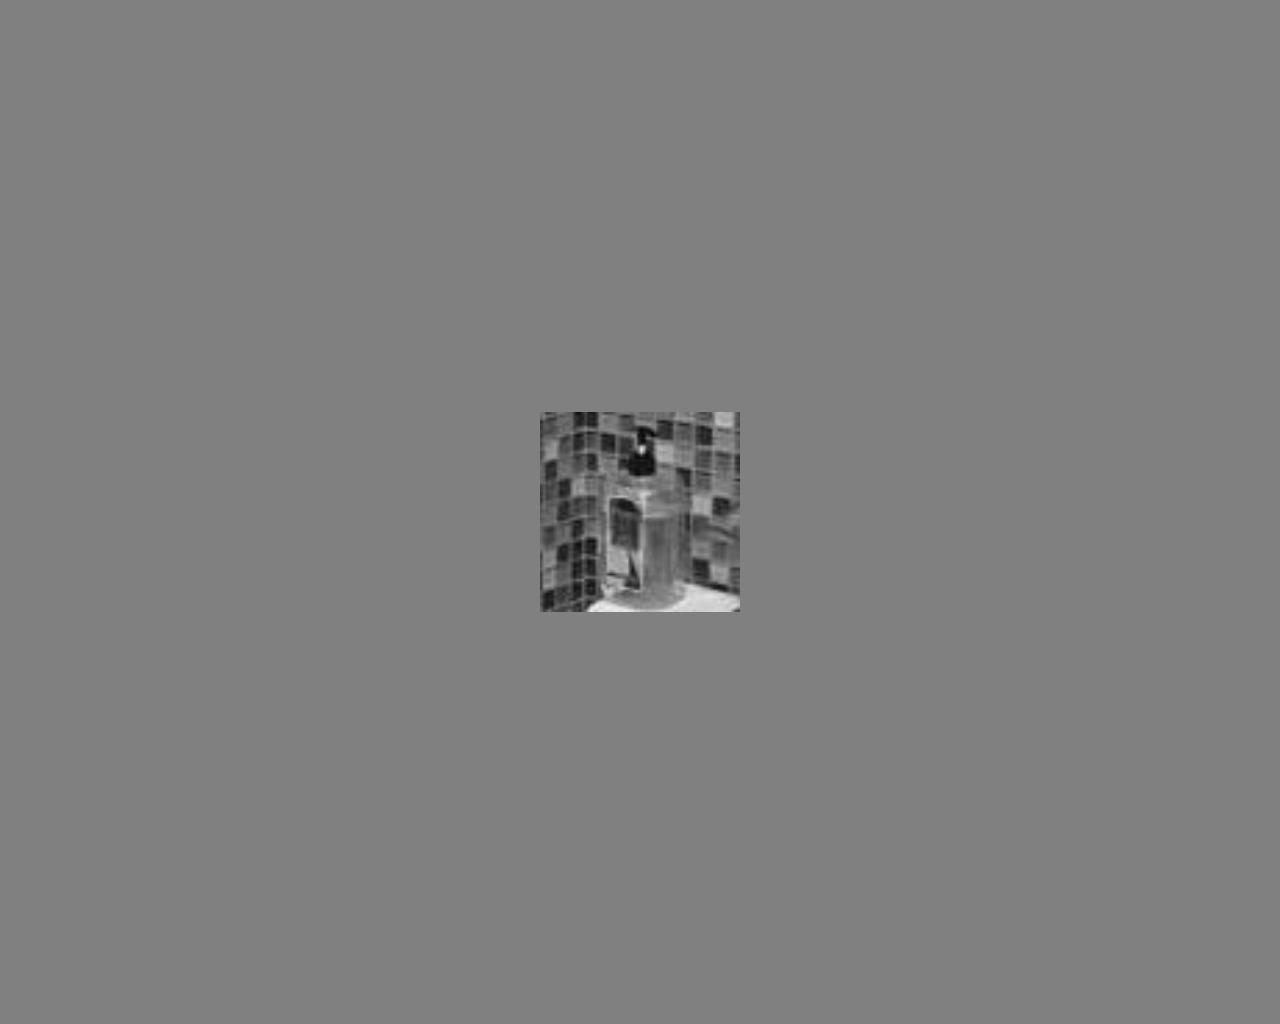
\includegraphics[width=\linewidth]{images/target_bathroom.jpg} 
        \caption{Muestra de target} \label{fig:expe-etapa-1}
    \end{subfigure}
    \hfill
    \begin{subfigure}[b]{0.32\textwidth}
        \centering
        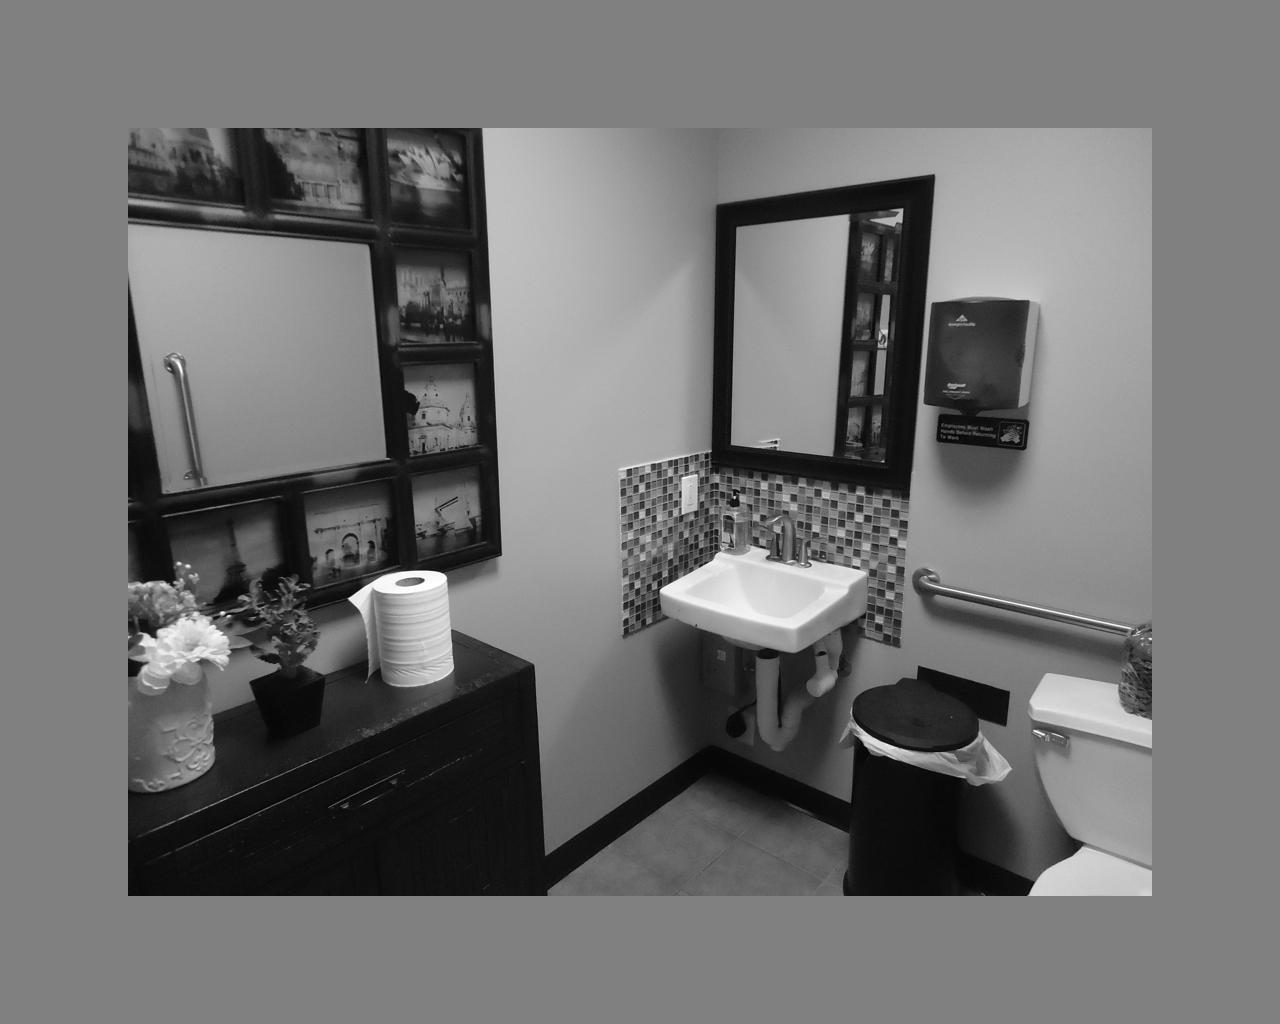
\includegraphics[width=\linewidth]{images/full_bathroom.jpg} 
        \caption{Imagen completa} \label{fig:expe-etapa-3}
    \end{subfigure}
    \hfill
    \begin{subfigure}[b]{0.32\textwidth}
        \centering
        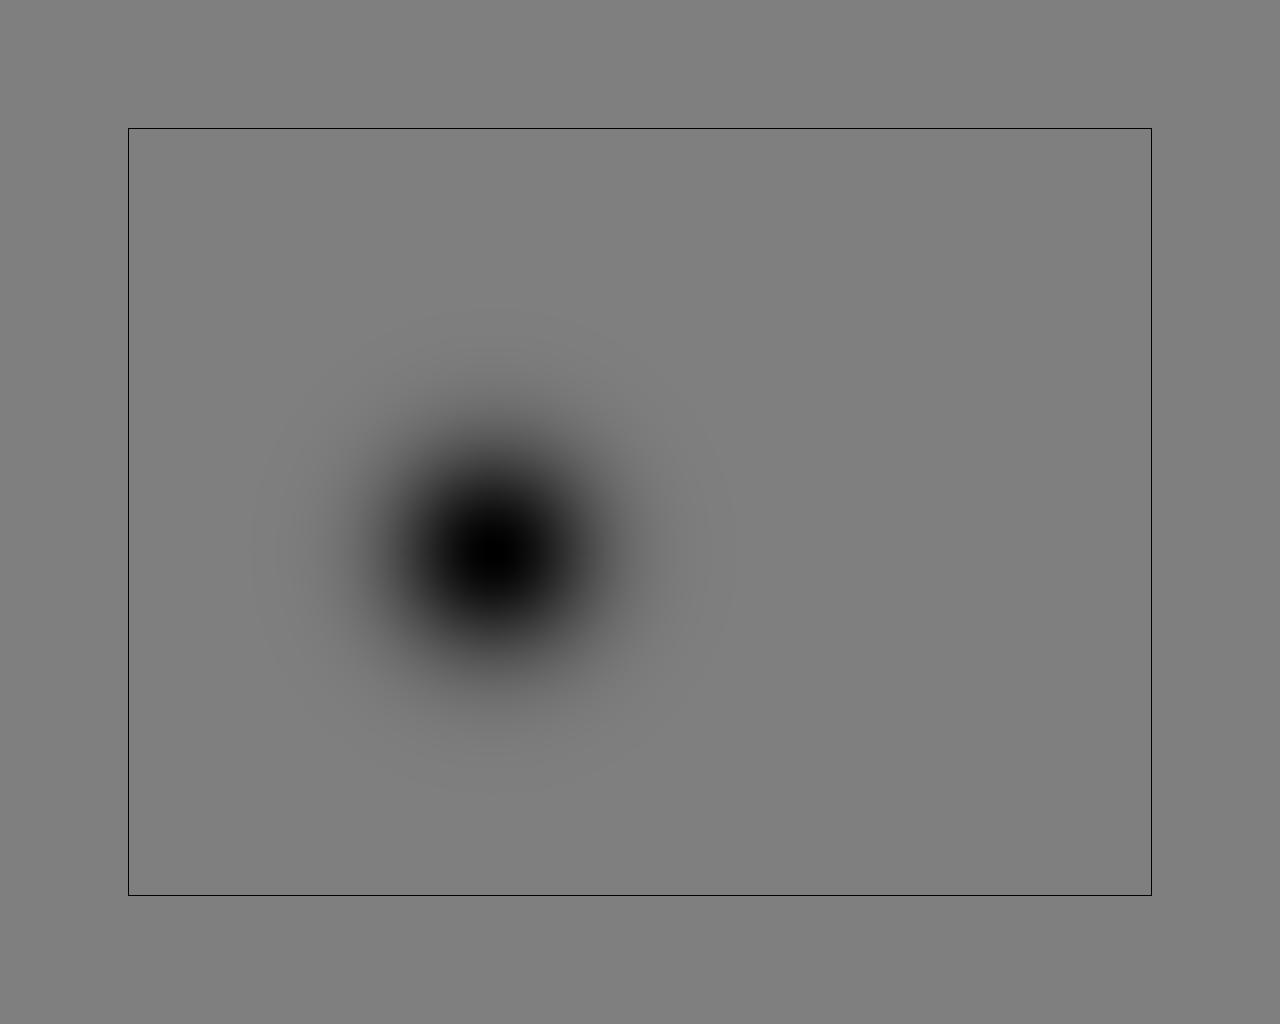
\includegraphics[width=\linewidth]{images/subjective_response_ahora.jpg} 
        \caption{Respuesta subjetiva} \label{fig:expe-etapa-4}
    \end{subfigure}
\end{figure}

Se fuerza a los sujetos a mirar en un punto negro a 300 píxeles del target. Este lugar varía por imagen pero es el mismo para todos los sujetos.

\end{frame}

\begin{frame}
\begin{itemize}
\item Según el ensayo elegimos aleatoriamente la cantidad de sacadas que se le permite realizar a las personas antes de cortar el ensayo y pedirle el reporte subjetivo. 
\item Elegir la distribución de cantidad de fijaciones no fue fácil, pues quisimos maximizar la cantidad de ensayos con varias fijaciones donde los sujetos no hayan encontrado el target.
\end{itemize}

\bigskip

\begin{table}[h]
\centering
\tiny
\begin{tabular}{c|c|c|c|c|c|c|c|c|c|}
\cline{2-10}
                                           & \multirow{2}{*}{\textbf{\tiny \begin{tabular}[c]{@{}c@{}} Cantidad \\ de sujetos\end{tabular}}} & \multirow{2}{*}{\textbf{\tiny \begin{tabular}[c]{@{}c@{}} Cantidad \\ de imágenes \end{tabular}}} & \multicolumn{7}{c|}{\textbf{Cantidad de sacadas}}                                        \\ \cline{4-10} 
                                           &                                                                                          &                                                                                                      & \textbf{2} & \textbf{3} & \textbf{4} & \textbf{8} & \textbf{12} & \textbf{16} & \textbf{64} \\ \hline
\multicolumn{1}{|c|}{\textbf{Tarea 1}}     & 3                                                                                        & 108                                                                                                  & 20,4\%    &            & 20,4\%    & 20,4\%    &             & 20,4\%     & 18,4\%     \\ \hline
\multicolumn{1}{|c|}{\textbf{Tarea 2}}     & 2                                                                                        & 108                                                                                                  & 25\%       &            & 25\%       & 25\%       &             & 12,5\%     & 12,5\%     \\ \hline
\multicolumn{1}{|c|}{\textbf{Tarea 3}}     & 6                                                                                        & 108                                                                                                  & 25\%       & 25\%       & 25\%       & 25\%       &             &             &             \\ \hline
\multicolumn{1}{|c|}{\textbf{Tarea final}} & 17                                                                                       & 134                                                                                                  & 13,4\%    &            & 14,9\%    & 29,9\%    & 41,8\%     &             &             \\ \hline
\end{tabular}
\caption{\label{tab:tareas} Distribuciones de cantidad de sacadas utilizadas en la puesta a punto del experimento.}
\end{table}


\end{frame}


\begin{frame}
\begin{itemize}
\item Tomamos datos de 30 participantes, pero 2 no pudieron ser grabados adecuadamente por un error del software.
\item De los 28 sujetos que obtuvimos, 3 fueron mujeres y 25 varones, todos ellos estudiantes o docentes de la FCEyN - UBA.
\end{itemize}

\bigskip
\bigskip

Como los target son de diferentes clases de objetos, notamos que para diseñar buenos algoritmos necesitábamos entender semánticamente a qué clase de objeto pertenece cada una. Para esto realizamos otro experimento.
\end{frame}

\subsection{Experimento de detección de objetos}
\begin{frame}{Experimento de detección de objetos}
\begin{itemize}
\item Mostramos cada uno de los target durante 3 segundos y luego le pedimos a los participantes que digan qué objeto es el de la imagen de tres formas distintas.
\item Los target se muestran en orden aleatorio, y son los mismos del experimento original.
\item Si el usuario no reconoce el objeto, existe una opción a ese fin.
\item Esta tarea se puede realizar online en varios días. Si quieren participar, sigue abierta en \texttt{http://objetos.gpoesia.com}
\item Obtuvimos datos de 17 participantes. No todos terminaron el experimento, pero tuvimos en promedio 10.5 respuestas por imagen.
\end{itemize}
\end{frame}

\section{Análisis del comportamiento}

\begin{frame}
En algunos ensayos la mirada se posó tan cerca del target (a menos de $1.25^{\circ}$ del centro) que llegó a fijar parte del mismo con la visión foveal. Por eso consideramos para nuestros análisis que el target en realidad fue encontrado aunque la vista no haya sido posada sobre el target.

\bigskip

Analizamos diferentes aspectos del experimento que utilizaremos más adelante, y mencionamos rápidamente.
\end{frame}


\begin{frame}{Longitud de las sacadas}
\begin{center}
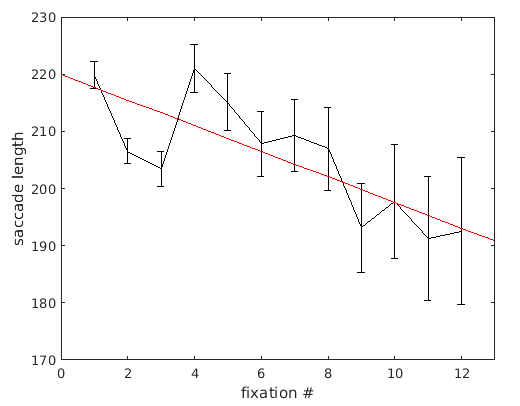
\includegraphics[width=0.6\textwidth]{images/mean-sacclen.png}
\end{center}

Vemos que la longitud de las sacadas decrece a lo largo del tiempo, consistentemente con otros trabajos.
\end{frame}

\begin{frame}{Sesgo de la fijación central}
\begin{center}
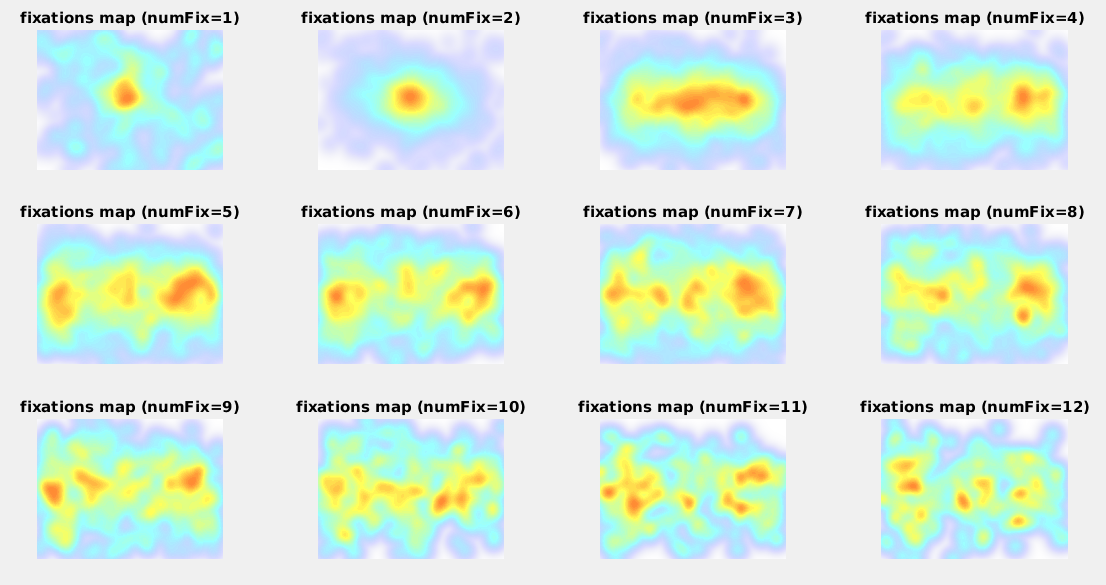
\includegraphics[width=0.9\textwidth]{images/heatmap-per-fix.png}
\end{center}

Notar que el sesgo también se marca en la primera fijación. \end{frame}

\begin{frame}
Notar que el sesgo también se marca en la primera fijación. Algunos sujetos movieron rápidamente los ojos desde la fijación pedida hacia el centro, y grabamos la primera fijación allí.

\begin{center}
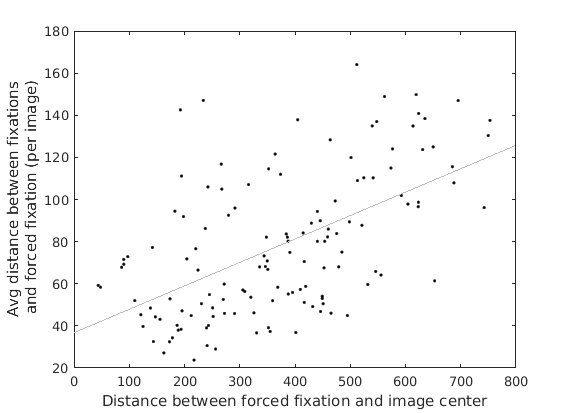
\includegraphics[width=0.6\textwidth]{images/scatter-first-fixation.png}
\end{center}

\bigskip

Se observa que la distancia del punto de la primera fijación al centro de la imagen correlaciona con cuán bien los participantes respetan la instrucción de mantener la mirada en el punto pedido.
\end{frame}

\begin{frame}{Cambios en incerteza según cantidad de fijaciones}
\begin{center}
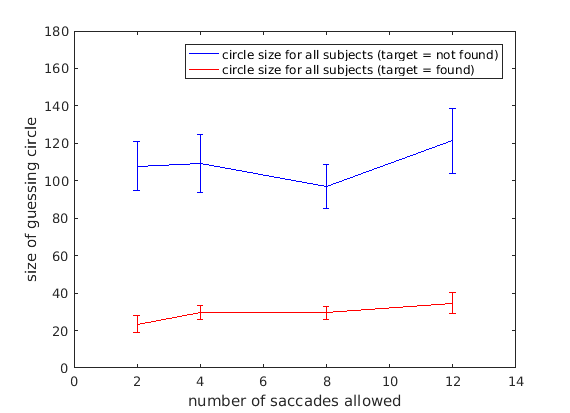
\includegraphics[width=0.6\textwidth]{images/mean_circle_size.png}
\end{center}

Además vimos en la tesis que existe un efecto "desmoralizador": si llevamos algunos ensayos sin encontrar el target, la probabilidad de colocar un círculo más grande se incrementa. Lo mismo vale pero en mucha menor medida para el caso opuesto (varios ensayos encontrando targets).
\end{frame}

% esto se puede saltear
\begin{frame}{Influencia de ensayos anteriores en la respuesta actual}
\begin{center}
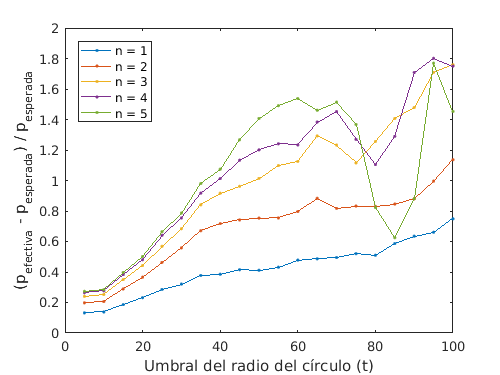
\includegraphics[width=0.6\textwidth]{images/desconfianza-rta-dif-relativa.png}
\end{center}
\end{frame}

\section{Modelos predictivos}
\begin{frame}
Ahora mostraremos los distintos modelos predictivos que proponemos. Estos modelos se dividen en dos clases según si predicen las regiones a ser fijadas (\textbf{modelos estáticos}) o si predicen el orden de las fijaciones (\textbf{modelos dinámicos}).
\end{frame}

\subsection{Modelos estáticos}

\begin{frame}
Crearemos nuestros propios modelos estáticos, basados en el mapa de saliencia creado por Judd. Lo compararemos con dos modelos del estado del arte, SAM y MLNet. 

\medskip
Si bien los mapas de saliencia no son predictores perfectos en tareas de búsqueda visual son buenos orientadores de la atención visual.

\bigskip
\bigskip
Antes de referirnos a cómo creamos los modelos tenemos que entender cómo vamos a medir su performance.
\end{frame}


\begin{frame}{Medidas de performance}

\begin{itemize}
{\small 
\item Tomamos los mapas de saliencia como un clasificador binario de los píxeles. Un porcentaje dado de los píxeles de una imagen se clasifican como positivos y el resto negativos.
\item Se grafica para varios porcentajes el True Positive Rate (TPR), que indica qué porción de las fijaciones caen en la región saliente.
}
\end{itemize}

\begin{figure}[b]
    \centering
    \begin{subfigure}[t]{0.3\textwidth}
        \centering
        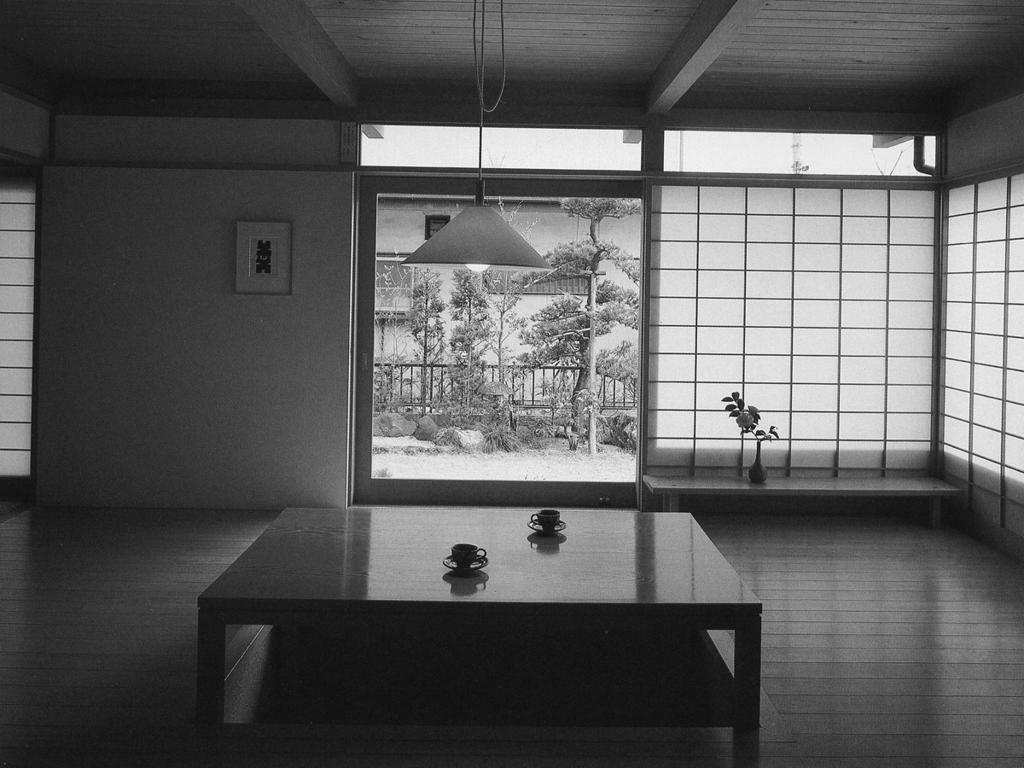
\includegraphics[width=\linewidth]{images/grayscale_100_oliva.jpg}
        \caption{\footnotesize Imagen original} \label{fig:grayscale_100_oliva}
    \end{subfigure}
    \hfill
    \begin{subfigure}[t]{0.3\textwidth}
        \centering
        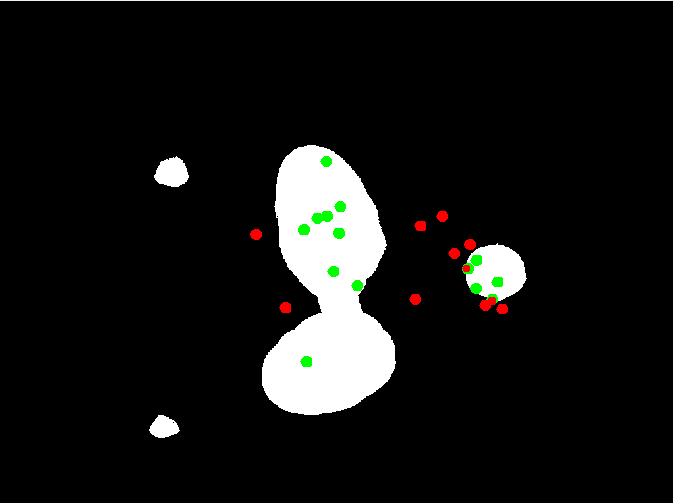
\includegraphics[width=\linewidth]{images/example-salient-percent-8-14.png} 
        \caption{\footnotesize 8.14\% más saliente de la imagen según SAM} \label{fig:example-salient-percent-8-14}
    \end{subfigure}
	\hfill
	\begin{subfigure}[t]{0.3\textwidth}
        \centering
        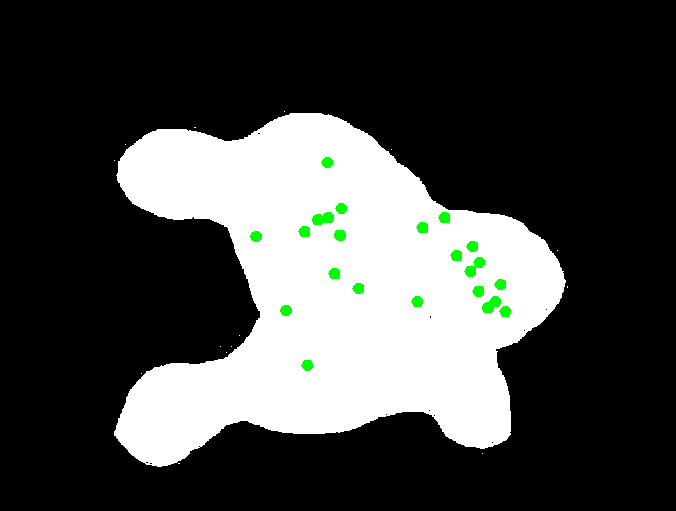
\includegraphics[width=\linewidth]{images/example-salient-percent-27-73.png} 
        \caption{\footnotesize
27.73\% más saliente de la imagen según SAM} \label{fig:example-salient-percent-27-73}
    \end{subfigure}
\end{figure}

\end{frame}

\begin{frame}{Modelos de saliencia como predictores de fijaciones}

\begin{figure}
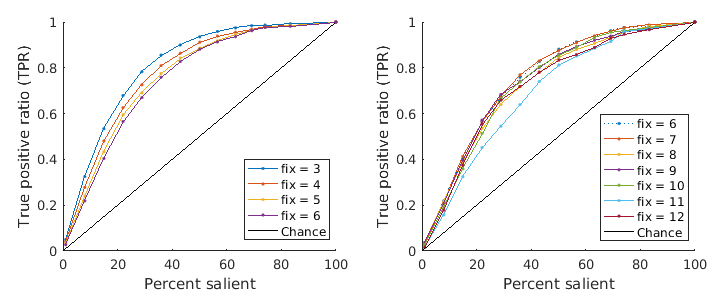
\includegraphics[width=\linewidth]{images/sam_all_fix_small.png} 
\caption{Performance de SAM}
\end{figure}

Tanto SAM como MLNet predicen mejor las primeras fijaciones que las últimas. Mostamos aquí solo SAM.

\bigskip

Veamos cómo es el modelo de Judd y como lo extenderemos para mejorar la performance recién mostrada.

\end{frame}

\begin{frame}{Modelo de saliencia de Judd}
\begin{itemize}
\item Se realiza un mapa de saliencia por imagen tomando las fijaciones de los humanos y suavizándolas con un filtro gaussiano. Este mapa es tomado como \textit{ground truth} para entrenar su modelo.
\item Para entrenar su modelo Judd toma 10 píxeles al azar del 20\% más saliente del mapa de saliencia  \textit{ground truth} y los identifica como píxeles salientes. Asimismo, toma 10 píxeles al azar del 30\% menos saliente y los toma como píxeles negativos.
\end{itemize}
\end{frame}

\begin{frame}{Modelo de saliencia de Judd (2)}
\begin{itemize}
\item Computa 33 features por imagen, que incluyen: mapas de colores (RGB), mapa de intensidad, mapa de orientación, mapa de contraste, mapa de distancia al centro de la imagen, mapa de distancia al horizonte, mapas de detección de rostros, autos, personas y dos mapas de saliencia base.
\item Luego entrena una Support Vector Machine (SVM) con las muestras positivas y negativas mencionadas anteriormente. Utiliza un kernel lineal por su simplicidad, y porque probó otros kernels pero no mejoró la performance.
\item \textbf{Este modelo permite muy fácilmente agregar y remover features} que se adapten mejor a nuestra tarea.
\end{itemize}
\end{frame}

\begin{frame}
\begin{itemize}
\item Tomaremos el modelo de Judd y lo adaptaremos a nuestra tarea, que es de búsqueda visual.
\item Removemos los features de rostros, autos, personas y los features de colores pues no aparecen en nuestra tarea.
\item Utilizamos SAM y MLNet como mapas de saliencia base, que son del estado del arte.
\bigskip
\item Extendemos Judd con dos tipos de mapas que extraen información del target:
\begin{enumerate}[I.]
\item Mapas teniendo en cuenta el aspecto netamente visual del target
\item Mapas teniendo en cuenta la semántica de la imagen mostrada. Esto incluye el reconocimiento de la clase de objeto a la que pertenece el target y la unión de este conocimiento con el de las experiencias previas del sujeto.
\end{enumerate}
\end{itemize}
\end{frame}

\begin{frame}{Extensión de Judd - tipo I}

\begin{itemize}
\item El primer mapa es del de la \textit{cross correlation} del target y la imagen original.
\item El segundo mapa intenta representar una \textbf{similitud de bajo nivel} entre el target y una porción de la imagen.
\end{itemize}

\begin{figure}
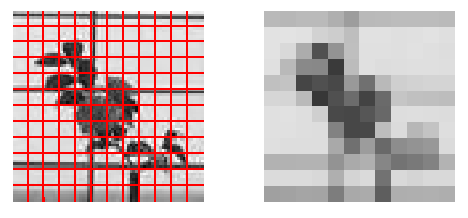
\includegraphics[width=0.7\linewidth]{images/grilla-gorda.png} 
\end{figure}

\end{frame}

\begin{frame}{Extensión de Judd - tipo II}
\end{frame}

\begin{frame}
\end{frame}

\begin{frame}
\end{frame}


\begin{frame}
\end{frame}




\section{Modelos dinámicos}
\begin{frame}
\end{frame}

\begin{frame}
\end{frame}


\end{document}
